\iffalse
\documentclass[journal,10pt,twocolumn]{article}
\usepackage{graphicx}
\usepackage[margin=0.5in]{geometry}
\usepackage[cmex10]{amsmath}
\usepackage{array}
\usepackage{booktabs}
\title{\textbf{Circle Assignment}}
\author{Bhavani Kanike}
\date{October 2022}

\providecommand{\norm}[1]{\left\lVert#1\right\rVert}
\providecommand{\abs}[1]{\left\vert#1\right\vert}
\let\vec\mathbf
\newcommand{\myvec}[1]{\ensuremath{\begin{pmatrix}#1\end{pmatrix}}}
\newcommand{\mydet}[1]{\ensuremath{\begin{vmatrix}#1\end{vmatrix}}}
\providecommand{\brak}[1]{\ensuremath{\left(#1\right)}}

\begin{document}

\maketitle
\paragraph{\textit{Problem Statement} \\\\-
\fi
Prove that the angle between the two tangents drawn from an external point to a circle is supplementary to the angle subtended by the line-segment joining the points of contact at the centre.
	\begin{figure}[!h]
		\centering
 \includegraphics[width=\columnwidth]{chapters/10/10/2/10/figs/circle1.pdf}
		\caption{}
		\label{fig:10/10/2/10}
  	\end{figure}
	\\
	\solution Follow the approach in Problem 
\ref{chapters/10/10/2/6}
for constructing the tangents to the circle.
\iffalse
}

\section*{\large Solution}

\section*{\large Construction}

\begin{figure}[h]
\centering
\includegraphics[width=1\columnwidth]{circle1.pdf}
\caption{Figure}
\label{fig:triangle}
\end{figure}

The dimensions of the figure is taken as below\\\\
{
\setlength\extrarowheight{2pt}
\centering
	\begin{tabular}{|c|c|}
	\hline
	\textbf{symbol}&\textbf{value}\\
	\hline
	Origin&(0,0)\\
	\hline
	r&4\\
	\hline
	h&(8,6)\\
	\hline
\end{tabular}
}
\\\\\\

TO PROVE :
\begin{equation}
	 \boldsymbol{\angle{AOB} + \angle{AhB} = 180^\circ}
\end{equation}\\
	The equation of a conic with directrix $\vec{n^Tx}$ = c , eccentricity e anf focus $\boldsymbol{f}$ is given by
	
\begin{equation}
	\vec{x}^T\vec{V}\vec{x} + 2\vec{u}^T + f = 0
\end{equation}
	for circle eccentricity e = 0 then,\\
\begin{equation}
	\vec{V} = \vec{I} = \myvec{1&0\\0&1} , \vec{u} = \myvec{0\\0} , f = -r^2
\end{equation}
Point q on conic is given by 
\begin{equation}
	\vec{q} = \vec{V}^{-1}(\vec{n} - \vec{u})
\end{equation}
where, $\vec{n}$ is the normal vectors of the tangents from a point h to the conic are given by 
\begin{equation}
	\vec{n} = \frac{\vec{e_1}}{\vec{e_1^T}h} + \mu_i\vec{Rh}
\end{equation}
\\
where $\mu _i$ 's are given by the following equation
\begin{equation}
	\mu_i = \frac{1}{\vec{m^TVm}}(-\vec{m^T(Vq+u)}	
\end{equation}
	 			$ \pm \sqrt{[\vec{m^T(Vq+u)}]^2 - (\vec{q^TVq + 2u^T }+ f)(\vec{m^TVm)}})$
\\\\
$\mu _i$ 's are obtained by substituting the following in equation 6\\\\
\begin{equation}
	\vec{m = Rh = \myvec{-2\\8}}  ;  \vec{u}  = \myvec{0\\0}  ;  \vec{q} = \frac{\vec{e_1}}{\vec{e_1^T}h}
\end{equation}
 R = $\myvec{-1&1\\1&0}$ 
\\\\
The obtained $\mu_i$'s are substituted in equation 5 and equation 5 is substituted in equation 6 the required points on conic A and B are obtained.\\\\
\section*{Calculation Part}
By Solving equation number 6 using equation number 7 parameters we will get two $\mu_i$ values\\
Therefore ,\\\\
$\mu_i$ =  $\pm 0.488525$\\\\

n1 is obtained by substituting $\mu_i$ = 0.488525\\
n2 is obtained by substituting $\mu_i$ = -0.488525\\

\begin{equation}
	\boldsymbol{n1} = \frac{\myvec{1\\0}}{\myvec{1\\0}^T\myvec{8\\6}} + \mu_1\myvec{0&-1\\1&0}\myvec{8\\6} = \myvec{-0.8\\3.9}
\end{equation}

\begin{equation}
	\boldsymbol{n2} = \frac{\myvec{1\\0}}{\myvec{1\\0}^T\myvec{8\\6}} + \mu_2\myvec{0&-1\\1&0}\myvec{8\\6} = \myvec{3.43\\-2.04}
\end{equation}

\begin{equation}
	\boldsymbol{A} = \myvec{\boldsymbol V}^{-1}\myvec{\boldsymbol{n_1-u}} = \myvec{-0.8\\3.9}
\end{equation}
\begin{equation}
	\boldsymbol{B} = \myvec{\boldsymbol V}^{-1}\myvec{\boldsymbol{n_2-u}} = \myvec{3.43\\-2.04}
\end{equation}
Now the point A and B are formed and tangents are drawn \\\\
To find the angle between AOB and AhB use inner product method \\

\begin{equation}
	\angle AOB = cos^{-1}\frac{(\vec{A}-\vec{O})^T(\vec{B}-\vec{O})}{\norm{(\vec{A}-\vec{O})}\norm{(\vec{B}-\vec{O})}}
\end{equation}\\
\begin{equation}
	\angle AOB = cos^{-1}\frac{\myvec{\myvec{-0.8\\3.9}-\myvec{0\\0}}^T \myvec{\myvec{3.43\\-2.04} - \myvec{0\\0}}}{\norm{\myvec{A-O}} \norm{\myvec{B-O}}}
\end{equation}

\begin{equation}
	\angle AOB = 2.32 radians = 2.32*\frac{180}{\pi} = 133^\circ
\end{equation}
\begin{equation}
	\angle AhB = cos^{-1}\frac{(\vec{h}-\vec{A})^T(\vec{h}-\vec{B})}{\norm{(\vec{h}-\vec{A})}\norm{(\vec{h}-\vec{B})}}
\end{equation}

\begin{equation}
	\angle AhB = cos^{-1}\frac{\myvec{\myvec{8\\6}-\myvec{-0.8\\3.9}}^T \myvec{\myvec{8\\6} - \myvec{3.43\\-2.04}}}{\norm{\myvec{h-A}} \norm{\myvec{h-B}}}
\end{equation}
\begin{equation}
	\angle AhB = 0.82 radians = 0.82*\frac{180}{\pi} = 47^\circ
\end{equation}
If $\angle AOB$ + $\angle AhB$ = 180$^\circ$ then \\
Angle AOB and angle AhB form a supplementary angle.
Therefore,
\begin{equation}
	\boldsymbol{\angle AOB + \angle AhB = 180^\circ}
\end{equation}
\begin{equation}
	\boldsymbol{133^\circ + 47^\circ = 180^\circ}
\end{equation}

\end{document}
\fi
